\documentclass[11pt]{article}
\usepackage[margin=1in]{geometry}
\usepackage{amsmath,amssymb}
\usepackage{graphicx}
\usepackage{booktabs}
\usepackage{xcolor}
\usepackage{fontspec}
\usepackage[colorlinks=true,linkcolor=blue,citecolor=blue,urlcolor=blue]{hyperref}
\usepackage{enumitem}
\newfontfamily\deva{Devanagari Sangam MN}[Script=Devanagari,Renderer=Harfbuzz]
\newcommand{\code}[1]{\texttt{#1}}
\newcommand{\flag}[1]{\texttt{<#1>}}

\title{\textbf{KupeFDX-hi-asr: A Streaming Hindi Speech Recognition and\\
Floor-Control System Fusing a Self-Supervised Omnilingual Encoder\\
with the Nandi-Mini Small Language Model}\\[4pt]
\large A Method Proposal}
\author{FrontiersMind / Kupe FDX --- Research}
\date{September 2026}

\begin{document}
\maketitle

\begin{abstract}
\noindent
We propose \textbf{KupeFDX-hi-asr}, a single streaming system for Hindi voice agents that
performs three tasks jointly: (i) accurate transcription, (ii) live domain-terminology
correction, and (iii) almost-full-duplex \emph{floor control} --- deciding \emph{when to
stay silent} and, rarely, when to emit a backchannel, a thinking-sound, or an
end-of-speech signal. The system fuses the \textbf{self-supervised (SSL) \code{omniASR\_W2V}} (wav2vec\,2.0) encoder
from Meta's Omnilingual ASR release~\cite{omni} --- using \emph{only} its SSL weights, not the
CTC-finetuned head --- with the Hindi-native \textbf{Nandi-Mini-150M} small language
model~\cite{nandi}. The architecture is encoder-agnostic, so FastConformer/IndicConformer
remains a one-flag fallback if Hindi WER stalls (Section~\ref{sec:enc}). \textbf{Nandi
produces the final transcript}; our own connectionist-temporal-classification (CTC)
head~\cite{ctc} is only a helper --- it fine-tunes the encoder on Hindi and supplies
end-of-speech timing, never the authoritative transcript, and none of Meta's CTC weights are
loaded. A projector maps continuous encoder features into Nandi's embedding space, and an
optional $k$-means quantizer can add discrete ``audio tokens'' to Nandi's vocabulary. Crucially, a dedicated
per-chunk floor-control head is trained so that its default, confident output is
\emph{NOTHING}: the model stays quiet on the overwhelming majority of chunks and emits a
signal only when it clearly fires. This document specifies the architecture, the
mathematics of every component and loss, the five-phase training schedule, the
audio-aware data-generation procedure with its scenario distribution and JSON formats, and
the streaming input/output contract. Per the request, results and conclusions are
deliberately excluded --- this is a method plan. All quantitative details below are drawn
directly from the reference implementation.
\end{abstract}

\section{Introduction and Motivation}
Production Hindi voice pipelines chain separate models for transcription, correction and
turn-taking. They sound robotic (dead silence while ``thinking''), miss domain terms, and
fire turn-boundary signals at the wrong moments. We instead fuse two open-weight
foundations into one proprietary system. The encoder is the \emph{raw self-supervised}
variant of Omnilingual ASR: it emits continuous contextual vectors and, having no baked-in
output vocabulary, sidesteps any tokenizer-mismatch problem~\cite{omni}. The decoder is
Nandi-Mini-150M, trained from scratch on 525\,B tokens across English and ten Indic
languages with native Devanagari coverage~\cite{nandi}, which supplies a strong Hindi
prior for correction and for generating natural backchannel words. The scope here is Hindi;
the design is deliberately built as a floor controller from the start so it validates on
one language before scaling to the remaining Indic languages plus English.

\section{Plain-Language Overview (for a new engineer)}
If you are new to speech ML, here is the whole project in everyday terms; every term is
defined again in detail later.
\begin{itemize}[leftmargin=1.4em,itemsep=1pt]
\item \textbf{The goal.} Build one model that, while a person speaks Hindi, (1) writes down
what they say, (2) fixes special words (medical/technical terms), and (3) decides \emph{when
to react} --- say a quick ``\deva हाँ'' (backchannel), make a thinking sound ``\deva हम्म'',
or detect that the person finished talking (end-of-speech). Most of the time it should
\emph{do nothing} except keep writing.
\item \textbf{Two ready-made models we glue together.} An \emph{encoder} (\code{omniASR\_W2V})
that turns sound into a list of number-vectors --- think of it as ``ears''. And a small
\emph{language model} (\code{Nandi-Mini-150M}) that is good at Hindi text --- think of it as
the ``mouth/brain''. The encoder does not know any words by itself; the language model does.
\item \textbf{The bridge.} A tiny neural layer called a \emph{projector} translates the
encoder's number-vectors into the ``language'' the SLM understands, and we feed them in as if
they were words. \textbf{Nandi (the SLM) writes the final transcript} --- not the encoder.
\item \textbf{The CTC head is a helper, not the writer.} We attach a simple \emph{CTC head}
(one linear layer) to the encoder, but only to (a) fine-tune the encoder on Hindi in Stage~A
and (b) detect where the silences/turn-ends are. It never produces the real transcript ---
that is always Nandi's job. (We also never load Meta's own CTC weights.)
\item \textbf{The flags.} We add five special words to the SLM's vocabulary:
\flag{BC} (backchannel), \flag{THINK}, \flag{EOS\_SPEECH} (end of speech), \flag{SILENCE},
and ``nothing''. A small \emph{floor-control head} predicts one of these for every short chunk
of audio; almost always the answer is ``nothing''.
\item \textbf{The data.} Normal speech datasets give us audio $+$ transcript. They do
\emph{not} tell us where the flags go. So we use an LLM (OpenAI \code{gpt-5.6-luna}) as a data
factory: we \emph{measure} the pauses in each audio clip and ask the LLM to place the flags
sensibly, producing labelled examples in JSON.
\item \textbf{Training in three stages.} We do not train everything at once.
\emph{Stage~A} --- fine-tune the ears (encoder) on Hindi. \emph{Stage~B} --- teach Nandi to
read the (now Hindi-tuned) encoder's audio and write the transcript. \emph{Stage~C} --- teach
the combined model the flags and word-correction. (Under the hood these are five resumable
training runs; Table~\ref{tab:phasedata} shows the data each uses.)
\item \textbf{How you run it.} Every step is one command (\code{commands.md}); a smoke test
(\code{bash run\_smoke.sh}) runs the entire pipeline on a laptop in seconds with tiny stand-in
models, so you can verify the wiring before spending GPU money. On the H100 you flip one config
flag (\code{backend: real}) and the same code loads the real models.
\end{itemize}

\section{Short Literature Review}
\textbf{Self-supervised encoders.} wav2vec\,2.0 learns speech representations by contrastive
prediction over masked latent frames~\cite{w2v2}; Omnilingual ASR scales this encoder to
7\,B parameters and covers 1{,}600+ languages, reporting character error rate (CER) below
10 for 78\% of them~\cite{omni}. Meta releases two decoders on top of the \emph{same
continuous} encoder: a CTC head that is ``a single linear layer\ldots optimized with a CTC
loss'', and an ``LLM-ASR'' transformer decoder that attains their best accuracy~\cite{omni}.
Notably, \emph{neither uses $k$-means or discrete units}; both consume continuous features.
\textbf{Discrete units} are a separate lineage: HuBERT derives targets by $k$-means
clustering of features~\cite{hubert}, which underpins textless speech-LM work but discards
acoustic detail. \textbf{Speech-to-LLM} systems such as Whisper's encoder-decoder~\cite{whisper},
Qwen-Audio~\cite{qwenaudio,qwen2audio} and SALMONN~\cite{salmonn} feed \emph{continuous}
audio features into a language model via a projector, which is the regime we adopt.
\textbf{Turn-taking} has been modelled by Voice Activity Projection, which predicts upcoming
speech activity to manage backchannels and turn shifts~\cite{vap}. \textbf{Indic ASR}
resources --- IndicWav2Vec~\cite{indicw2v} and the 6{,}400\,h Shrutilipi corpus~\cite{shrutilipi}
--- make thousands of hours of Hindi available. Our contribution is to \emph{fuse} a raw
Omnilingual encoder with a Hindi-native SLM into one streaming system that transcribes,
corrects, and controls the floor, with an explicit stability guarantee against over-firing.

\section{System Overview}
Figure~\ref{fig:arch} shows the single forward path. Audio is denoised and passed through
the causal SSL encoder. Its continuous features fan out to (a) the CTC head, (b) the
projector that produces 832-dimensional soft prompts for Nandi, (c) an optional $k$-means
quantizer producing discrete audio-code tokens, and (d) the per-chunk floor-control head.
Nandi autoregressively decodes the corrected transcript with inline control signals,
conditioned on a domain tag and rolling conversation context.

\begin{figure}[h]\centering
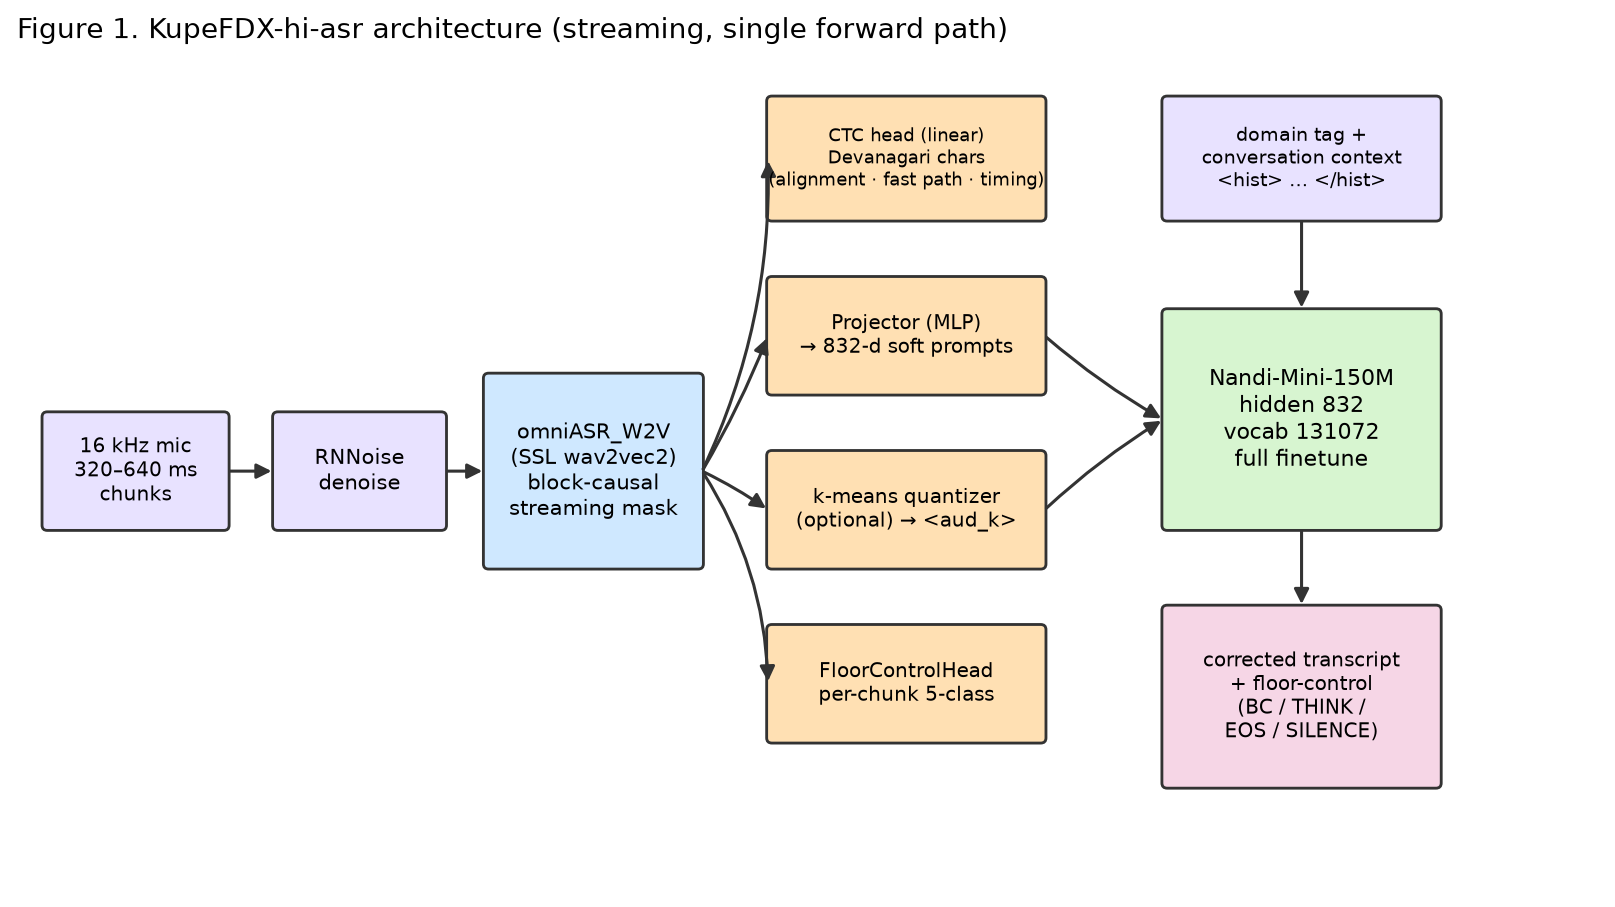
\includegraphics[width=\linewidth]{figs/fig_arch.png}
\caption{KupeFDX-hi-asr architecture. The encoder is used in a block-causal (streaming)
mode; the CTC head is retained for the whole project.}
\label{fig:arch}
\end{figure}

\section{Encoder and Streaming (Block-Causal) Masking}\label{sec:enc}
The encoder $\mathrm{Enc}$ maps a waveform $x$ (16\,kHz mono) to features
$H=\mathrm{Enc}(x)\in\mathbb{R}^{T\times D}$ at a frame rate of $50$\,fps (hop $320$
samples). To make the \emph{validated} word error rate a genuine streaming number rather
than an offline one we later regress, we impose a block-causal attention mask from the
first phase. With chunk size $C$ frames and left context of $L$ chunks, define the chunk
index $c(i)=\lfloor i/C\rfloor$; the additive mask is
\begin{equation}
M_{ij}=\begin{cases}0 & \text{if } c(i)-L \le c(j) \le c(i),\\ -\infty & \text{otherwise.}\end{cases}
\end{equation}
Thus frame $i$ attends only within its own chunk and the $L$ preceding chunks, never to the
right. In the reference configuration $C{=}32$ frames ($\approx 640$\,ms) and $L{=}2$. A unit
test verifies no future leakage: perturbing the last $\sim$200\,ms of audio leaves earlier
frame outputs unchanged. The encoder wrapper exposes a stable interface
$\big(H,\,\ell\big)=\mathrm{Enc.features}(x)$ with per-clip frame lengths $\ell$, so the raw
Omnilingual backbone (\code{backend: real}) and a small stand-in used for testing are
interchangeable.

\paragraph{Which encoder, and the SSL-only rule (important).} We use the \textbf{Omnilingual
\code{omniASR\_W2V} encoder}, and we use \textbf{only its self-supervised (SSL) wav2vec\,2.0
weights}. We do \emph{not} load Meta's CTC-finetuned checkpoint (\code{omniASR-CTC-*}) or any
of its decoder/head weights --- we attach and train \emph{our own} CTC head (Section~\ref{sec:ctc})
from scratch in Phase 1. The SSL encoder has no output vocabulary baked in, which is exactly
why it composes cleanly with Nandi and our fresh CTC head (no tokenizer mismatch). The loader
(\code{encoders.py}) refuses a \code{*-CTC-*} id to make this rule impossible to violate by
accident.

\emph{Honest risk note.} Two independent 2026 real-world Hindi benchmarks measure the
\emph{full} Omnilingual ASR system as weaker than FastConformer/IndicConformer on Hindi ---
Vaani~\cite{vaani}: $26.4$ WER for \code{omniASR\_LLM\_1B} vs $10.6$/$14.2$ for
FastConformer/IndicConformer; Voice-of-India~\cite{voi}: $13.7$--$14.9$ vs $8.2$. Those numbers
are for Meta's \emph{off-the-shelf} system, not for our recipe (a Hindi-fine-tuned SSL encoder
$+$ our CTC head $+$ Nandi correction), so they are a documented risk, not a verdict on our
design. Because the architecture is encoder-agnostic (the projector adapts any encoder width),
\textbf{FastConformer/IndicConformer is a one-line fallback} (\code{encoder\_type: fastconformer})
if Phase-3 Hindi WER stalls above target. Everything else in this proposal is unchanged by the
swap. (See \code{ENCODER\_DECISION.md} for the full measured comparison.)

\paragraph{How much audio reaches the SLM, and how (Figure~\ref{fig:audioflow}).} A $640$\,ms
streaming chunk of $16$\,kHz mono audio is $10{,}240$ samples. The omniASR\_W2V SSL encoder
turns it into $32$ frames ($20$\,ms/frame, $50$\,fps), each a \emph{continuous} vector. The
projector maps each frame to one $832$-d soft prompt, so Nandi receives $32$ continuous
$832$-d vectors per chunk (FastConformer would give $8$), wrapped in
\code{<audio>\,\ldots\,</audio>} and fed as \code{inputs\_embeds}. Nothing is discretized. A
rolling buffer plus the block-causal mask (left context $2$ chunks) makes this a true streaming
forward.
\begin{figure}[h]\centering
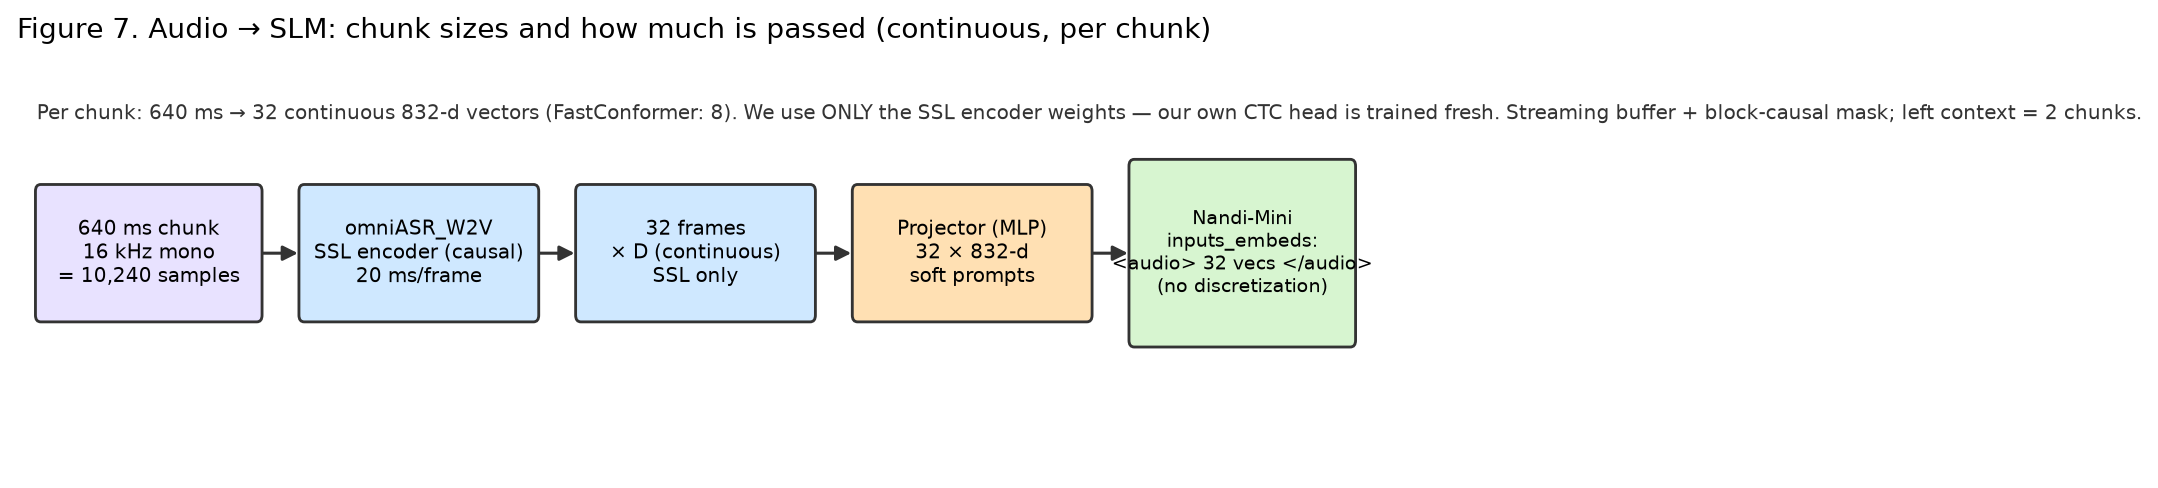
\includegraphics[width=\linewidth]{figs/fig_audioflow.png}
\caption{Per-chunk audio $\to$ SLM: $640$\,ms $\to$ $32$ continuous $832$-d soft prompts
(omniASR\_W2V SSL; FastConformer would give $8$).}
\label{fig:audioflow}
\end{figure}

\section{The CTC Head: Continuous Features, No $k$-means}
\label{sec:ctc}
Following Omnilingual's CTC recipe~\cite{omni}, the head is a single linear map from the
$D$-dimensional continuous features to a Devanagari character vocabulary of size $V_c$
(index $0$ is the CTC blank), followed by a log-softmax. For target character sequence $y$
and input length $T$, the CTC loss marginalizes over all frame-level alignments $\pi$ that
collapse (remove repeats, then blanks) to $y$:
\begin{equation}
\mathcal{L}_{\text{CTC}}=-\log\!\!\sum_{\pi\in\mathcal{B}^{-1}(y)}\ \prod_{t=1}^{T} p(\pi_t\mid H).
\end{equation}
\textbf{The CTC head is a helper, not the transcript producer.} Its purpose is (a) to be the
objective that fine-tunes the Omni SSL encoder on Hindi in Stage~A, (b) a monotonic-alignment
anchor that speeds Nandi's convergence and curbs hallucination, and (c) a free
end-of-speech/silence \emph{timing} signal --- a long run of CTC-blank frames at the tail
marks a probable turn end. \textbf{The final transcript always comes from Nandi}
(\code{model.generate}); the greedy CTC string is at most a throwaway low-latency draft
(off by default in streaming). This also answers whether $k$-means is needed: it is not ---
the self-supervised continuous encoder plus a linear CTC head is enough to adapt the encoder,
with no discretization, exactly as in Meta's release. We never load Meta's CTC weights; our
head is trained from scratch.

\section{Projector and Optional Discrete Audio Tokens}
The projector (a two-layer MLP with LayerNorm and a GELU nonlinearity) maps each continuous
frame to Nandi's input width $E{=}832$, and owns two learned marker vectors
$\langle\text{audio}\rangle,\langle/\text{audio}\rangle$. These continuous soft prompts are
the primary way Nandi ``hears'' the encoder --- the same continuous-feature regime used by
SALMONN and Qwen-Audio~\cite{salmonn,qwenaudio}, and by Omnilingual's own LLM-ASR
decoder~\cite{omni}, and the recommended default.

To additionally give Nandi \emph{discrete} audio tokens (so that acoustic units live in the
same embedding table as text), we optionally quantize features with $k$-means. Fitting
solves Lloyd's objective over a feature sample $\{f_n\}$ with $K$ centroids $\{\mu_k\}$,
\begin{equation}
\min_{\{\mu_k\}}\ \sum_{n}\ \big\lVert f_n-\mu_{a(n)}\big\rVert_2^2,\qquad a(n)=\arg\min_k \lVert f_n-\mu_k\rVert_2^2,
\end{equation}
and each frame is encoded to its nearest centroid index, surfaced as a vocabulary token
$\flag{aud\_k}$. Because discretization discards acoustic detail, we treat it as an additive
ablation ($K{=}2048$ when enabled, $0$ by default); residual vector quantization is a natural
stronger alternative if discrete tokens prove useful. The recommendation is therefore:
\emph{use continuous soft prompts as the primary signal; add $k$-means audio tokens only if
an ablation shows they help.}

\section{The Nandi Decoder, Token Extension, and Tokenizer Fertility}
Nandi-Mini-150M is a decoder-only transformer with hidden size $832$, a BPE vocabulary of
$131{,}072$ with native Devanagari, $16$ layers applied with layer-sharing ($\times 2$),
grouped-query attention ($16$ query / $4$ key-value heads), SwiGLU, RMSNorm, rotary position
embeddings ($\theta{=}10^5$), a $2048$-token context, tied input/output embeddings, and a
\emph{factorized} embedding of rank $196$~\cite{nandi}. Audio enters as \code{inputs\_embeds},
so Nandi's text vocabulary is never resized for text; we extend it only by a small set of
new tokens: the audio and history markers, the floor-control flags, and (optionally) the
$K$ audio-code tokens. Extension appends rows to the factorized embedding table
$W\in\mathbb{R}^{V\times 196}$ and, because the head is tied, both input and output sides
grow consistently; each new row is initialized to the mean of existing rows plus small
noise. This is the single riskiest piece of the fusion and is covered by a unit test that
runs on a faithful structural mirror (and, where reachable, on the real model).

\paragraph{Tokenizer fertility.} Fertility is the mean number of subword tokens per word,
\begin{equation}
\mathcal{F}=\frac{\#\text{subword tokens}}{\#\text{words}},
\end{equation}
measured on a representative Hindi set by \code{scripts/08\_tokenizer\_fertility.py}. Lower
fertility means shorter target sequences, faster decoding, and more of Nandi's $2048$-token
budget left for audio soft prompts and conversation context. A native-Devanagari BPE such as
Nandi's is expected to fragment Hindi far less than a character-level baseline (whose
fertility upper-bounds at the characters-per-word count); the script reports the measured
value together with characters-per-token and bytes-per-token.

\paragraph{Sequence layout.} Figure~\ref{fig:seq} shows the sequence assembled per example:
an optional context prefix, then \code{bos}, the audio markers wrapping the projected frames
(and any audio-code tokens), then the supervised target. The prefix is masked out of the
loss (label $-100$).
\begin{figure}[h]\centering
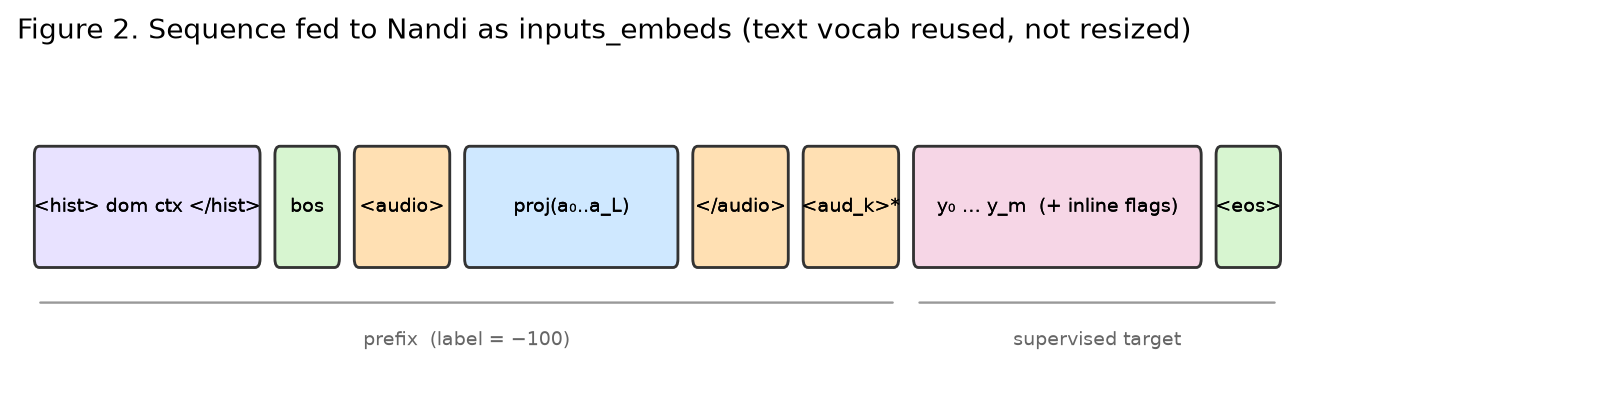
\includegraphics[width=\linewidth]{figs/fig_seq.png}
\caption{Token sequence fed to Nandi as continuous embeddings; only the target span is
supervised.}
\label{fig:seq}
\end{figure}

\section{Floor Control: Inline Flags and a Stable Per-Chunk Head}
\label{sec:fc}
Four mutually exclusive signals are defined with non-overlapping semantics:
\flag{EOS\_SPEECH} (the user turn is genuinely finished --- semantic completeness \emph{and}
a real trailing pause), \flag{BC} (a short listener acknowledgment \emph{while the user is
still speaking}, carrying a surface word such as \deva हाँ), \flag{THINK} (a filler while
the \emph{system} composes a reply, only \emph{after} \flag{EOS\_SPEECH}, e.g. \deva हम्म),
and \flag{SILENCE} (a sustained low-speech stretch that is not a turn boundary). The absence
of any flag denotes \emph{nothing happens}.

\paragraph{Inline representation.} In the autoregressive target, a flag is written
\emph{only at the moment it occurs}; there is no per-frame \flag{NOP}. A backchannel renders
as ``\flag{BC} \deva हाँ''; end-of-speech as ``\flag{EOS\_SPEECH}''; an ordinary or
mid-utterance pause renders \emph{nothing}. This absence is the core defence against
over-firing: a mid-sentence pause is present in the audio features but carries no flag in the
target, teaching restraint. During floor-control training the inline flag positions are
up-weighted so that rare signals are learnable without the no-flag majority drowning them:
with the set of flag positions $\mathcal{S}$,
\begin{equation}
\mathcal{L}_{\text{fc}}^{\text{inline}}=\frac{1}{|\mathcal{S}|}\sum_{t\in\mathcal{S}} -\log p(y_t\mid y_{<t}).
\end{equation}

\paragraph{Per-chunk head (the streaming stability layer).} A streaming agent is queried
every chunk, and the answer must be \emph{no} most of the time. A dedicated head classifies
each chunk into one of five classes
$\{\text{NOTHING},\flag{BC},\flag{THINK},\flag{EOS\_SPEECH},\flag{SILENCE}\}$. The
\flag{BC} surface may be a plain acknowledgment (\deva हाँ, अच्छा, जी) \emph{or} an emotional
expression --- laughter \deva हाहाहा, a sigh \deva उफ़, surprise \deva ओह/अरे --- generated by
Nandi when the context warrants it. Encoder frames
in chunk $c$ are mean-pooled to $\bar h_c$ and scored by a two-layer MLP; training minimizes
a class-weighted cross-entropy
\begin{equation}
\mathcal{L}_{\text{fcc}}=-\sum_{c} w_{y_c}\,\log p(y_c\mid \bar h_c),\qquad
w=(0.3,\,2,\,2,\,2,\,2),
\end{equation}
where labels come from the timeline: every \emph{ordinary ASR chunk is a NOTHING label}, so
NOTHING dominates the data and the head \emph{learns to stay quiet}; the weights up-weight
the rare classes only enough to keep them learnable. This head already receives the NOTHING
baseline in Phase~3 (weight $0.2$ on pure-ASR chunks) before Phase~4 adds the rare events.

\paragraph{Inference guard.} At run time a decider adds two hard guards on top of the
softmax $p$ at chunk $c$ (Figure~\ref{fig:stream}). It emits class $k^\star=\arg\max_k p_k$
only if
\begin{equation}
p_{k^\star} > \tau_{k^\star}\quad\text{and}\quad p_{k^\star} > p_{\text{NOTHING}},
\end{equation}
with thresholds $\tau=0.5$ for \flag{BC}/\flag{THINK}/\flag{EOS\_SPEECH} and $\tau=0.6$ for
\flag{SILENCE}; additionally \flag{BC}/\flag{THINK} require a minimum gap of $3$ chunks since
the last fire (anti-chatter), and \flag{EOS\_SPEECH} latches until the turn resets. Thus even
if logits wobble the system cannot fire on every chunk --- the quiet default holds by
construction.

\paragraph{Controllable at inference (the temperature analog).} Firing is a dial, not a
fixed policy. A \code{StreamControls} object exposes, per signal, a probability threshold, a
logit \emph{bias} (eagerness: $+$ fires more, $-$ suppresses), a minimum chunk gap, and an
on/off switch, plus a global softmax temperature $\tau_{\text{soft}}$ scaling
$z\!\to\!z/\tau_{\text{soft}}$ before the decision. An operator can thus make the agent
backchannel more (raise $\text{bias}[\flag{BC}]$), commit to end-of-turn more conservatively
(raise $\tau_{\flag{EOS\_SPEECH}}$), or disable thinking-sounds --- all at inference, without
retraining. The \emph{word} is decoupled from the \emph{decision}: the head decides
\emph{when}; Nandi generates the surface (an acknowledgment or an emotional expression) after
the flag in the autoregressive pass.
\begin{figure}[h]\centering
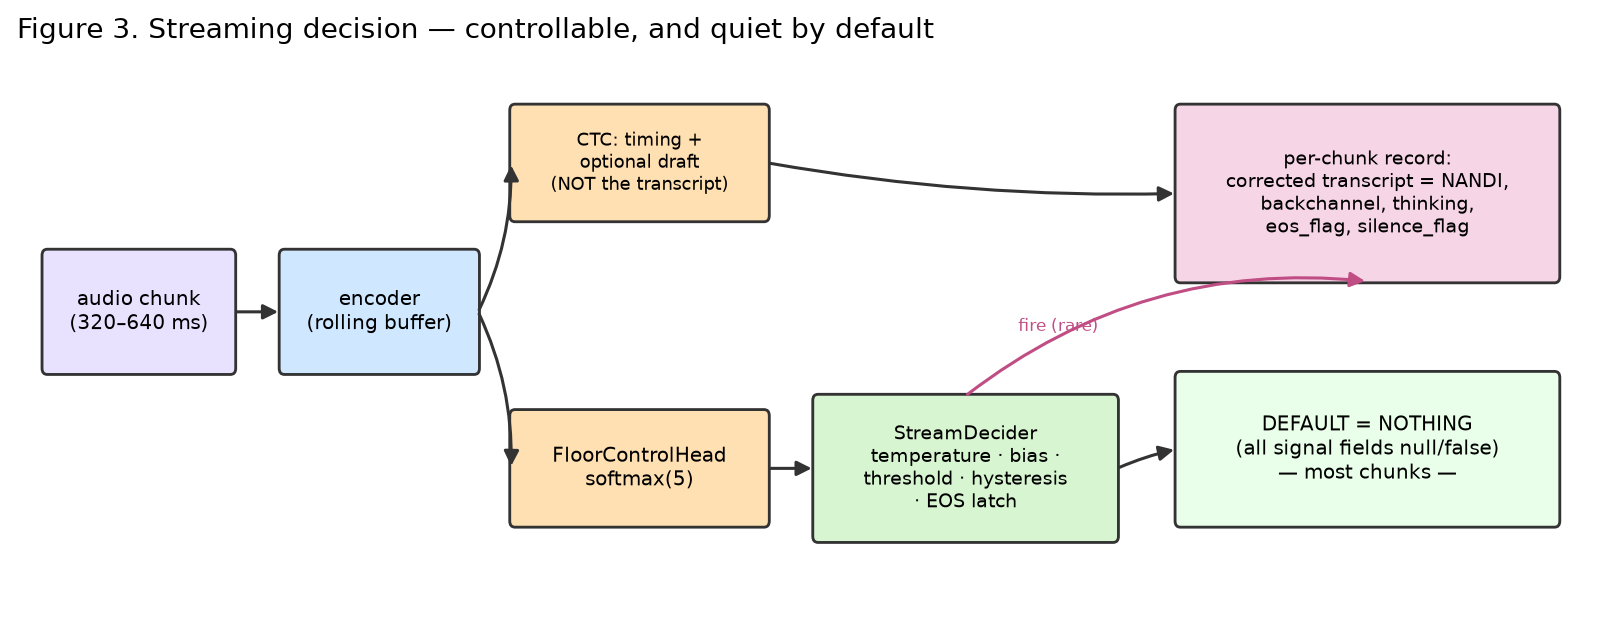
\includegraphics[width=\linewidth]{figs/fig_stream.png}
\caption{Per-chunk streaming decision. Most chunks return NOTHING (all signal fields
null/false); a signal is emitted only when it clearly fires.}
\label{fig:stream}
\end{figure}

\section{Training Objective}
The total loss combines four terms with phase-dependent weights:
\begin{equation}
\mathcal{L}=\lambda_{\text{lm}}\,\mathcal{L}_{\text{lm}}
+\lambda_{\text{ctc}}\,\mathcal{L}_{\text{CTC}}
+\lambda_{\text{fc}}\,\mathcal{L}_{\text{fc}}^{\text{inline}}
+\lambda_{\text{fcc}}\,\mathcal{L}_{\text{fcc}},
\end{equation}
where $\mathcal{L}_{\text{lm}}=-\sum_t \log p(y_t\mid y_{<t},\text{prefix})$ is the standard
next-token cross-entropy over the supervised target span. Optimization uses AdamW with a
cosine schedule and linear warmup, bf16 on the H100, gradient clipping, and a low-learning-rate
parameter group for the encoder when it is unfrozen. Training is fully resumable: a checkpoint
bundles model, optimizer, scheduler, global step and RNG state.

\section{Training: Three Stages (Five Runs)}
Training is organised as three stages, implemented as five resumable runs
(Figure~\ref{fig:phases}). \textbf{Stage~A (run 1)} fine-tunes the Omni SSL encoder on Hindi
using our CTC head as the objective --- this is the ``teach the encoder more Hindi'' step, and
the CTC head is only a training tool here, not the final transcript. \textbf{Stage~B (runs
2--3)} teaches Nandi to transcribe from the adapted encoder's audio (the projector aligns the
audio to Nandi's space, then everything is fine-tuned jointly; run 3 is the main $<5\%$ WER
gate, and \emph{Nandi} produces the transcript). \textbf{Stage~C (runs 4--5)} adds the
floor-control signals and domain-term correction on the combined model. Each run sets which
sub-modules train and the loss weights, following the schedule in the implementation.
\begin{table}[h]\centering\small
\begin{tabular}{@{}llll@{}}
\toprule
Phase & Trains & Frozen & Loss weights $(\lambda_{\text{lm}},\lambda_{\text{ctc}},\lambda_{\text{fc}},\lambda_{\text{fcc}})$\\
\midrule
1 CTC          & encoder, CTC head              & ---                         & $(0,\,1,\,0,\,0)$\\
2 Align        & projector, Nandi               & encoder, CTC               & $(1,\,0.3,\,0,\,0)$\\
3 Joint        & all (encoder low-LR)           & ---                         & $(1,\,0.3,\,0,\,0.2)$\\
4 Floor-control& projector, Nandi, FC head      & encoder, CTC               & $(1,\,0.1,\,3,\,1)$\\
5 Domain       & Nandi                          & encoder, projector, CTC    & $(1,\,0.1,\,1,\,0)$\\
\bottomrule
\end{tabular}
\caption{Phase schedule. Phase 3 is the main $<5\%$ streaming-WER gate; it also pre-trains
the per-chunk head on the NOTHING baseline before Phase 4 introduces rare events. Nandi is
\emph{fully} fine-tuned (single H100).}
\end{table}
\begin{figure}[h]\centering
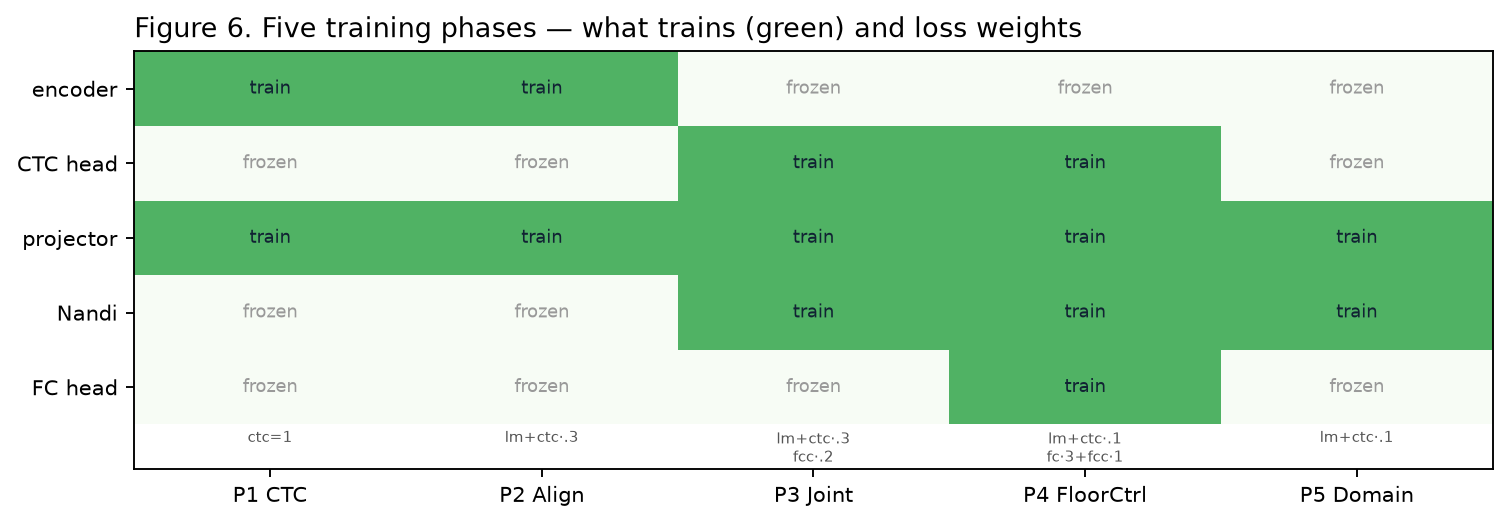
\includegraphics[width=0.82\linewidth]{figs/fig_phases.png}
\caption{What trains (green) versus frozen per phase, with the loss weights.}
\label{fig:phases}
\end{figure}
The mental model: Phases 1--3 teach transcription and how to ``understand'' the encoder's
audio (continuous soft prompts, and optionally discrete audio tokens); Phase 4 post-trains
the flags with transcription context; Phase 5 adds domain-term correction. Phases 4--5 always
mix in ASR data to prevent forgetting.

\paragraph{What data goes in and comes out of each run.} Table~\ref{tab:phasedata} is the
single most useful reference for an implementer: for every run it names the stage, the exact
input, the supervised target (what the model is trained to output), and the data file used.
\begin{table}[h]\centering\small
\begin{tabular}{@{}p{0.5cm} p{1.7cm} p{3.1cm} p{4.0cm} p{2.7cm}@{}}
\toprule
Stg & Run & Input (per example) & Target / output (supervised) & Data used\\
\midrule
A & 1 CTC & raw audio waveform & Devanagari \emph{characters} (CTC) --- adapts the encoder, not the final transcript & ASR ($\approx$2{,}500\,h)\\
B & 2 Align & audio (cached features) $+$ that clip's transcript & transcript \emph{tokens} (Nandi decodes them) & same ASR data\\
B & 3 Joint & raw audio & transcript tokens ($+$ CTC aux) --- \textbf{Nandi is the transcript} & ASR $2{,}500$\,h $+$ domain $400$\,h\\
C & 4 Floor & audio $+$ context $+$ domain tag & \code{target\_sequence} $=$ transcript with \emph{inline flags}; $+$ per-chunk flag label (mostly ``nothing'') & \code{fc.jsonl} ($\approx$300\,h) $+$ mixed ASR\\
C & 5 Domain & audio $+$ context $+$ domain tag & \emph{corrected} transcript (domain terms fixed) & \code{domain.jsonl} ($\approx$400\,h)\\
\bottomrule
\end{tabular}
\caption{Per-phase training data: input, supervised target, and source file. In every phase
the audio is the input; only the \emph{target} and the trainable modules change. Phase 1
targets characters (CTC); Phases 2--5 target Nandi tokens; Phase 4 adds inline flags and the
per-chunk floor-control label; Phase 5 changes the target from the raw to the corrected
transcript.}
\label{tab:phasedata}
\end{table}

\paragraph{Expectations (what ``done'' looks like, and the risks).} This is a proposal, so no
results are claimed; the targets we hold ourselves to are: Phase 1 encoder greedy-CTC WER
$<\!\sim\!9\%$; Phase 3 the main gate --- \textbf{streaming AR WER $<5\%$} on a clean blind
test (with $\approx$3{,}200\,h of quality-filtered data); Phase 4 floor-control $F_1>0.8$ per
signal with a false-fire rate $<2\%$ on no-flag examples; Phase 5 higher domain-term accuracy
with no WER regression. Realistic caveats an implementer should expect: (i) data quality
dominates volume past $\sim$1.5\,k\,h --- noisy $5$\,k\,h loses to clean $2.5$\,k\,h; (ii) if
Phase-3 WER stalls at $6$--$7\%$, the lever is \emph{more clean data / harder filtering}, not
more epochs; (iii) the Omni SSL encoder is a bet (see the honest risk note in Section~\ref{sec:enc})
--- if Hindi WER will not drop, switch the encoder to FastConformer with one config flag; (iv)
the floor-control model must see far more ``nothing'' than signals or it will over-fire ---
this is enforced by the data distribution and the inference guards.

\section{Data: Hours, Sources, and Generation}
\paragraph{Budget.} We target $\approx$3{,}200 curated hours (Figure~\ref{fig:hours}):
2{,}500\,h core clean ASR, 400\,h domain packs (medical / technical / support / general),
and 300\,h floor-control. Because the SSL backbone is already massively multilingually
pretrained and Nandi supplies a strong decoder prior, quality-filtered data at this scale is
the realistic path to $<5\%$ streaming Hindi WER (data quality dominates volume past
$\sim$1.5\,k\,h). Public sources include Shrutilipi~\cite{shrutilipi}, IndicVoices, Kathbath,
Vaani, Spring-INX, MUCS, Common Voice, and FLEURS; the cleanest $\sim$2.5\,k\,h are selected
by a quality filter. A held-out dev set (15--20\,h) and blind multi-domain test sets
($\approx$25\,h) are frozen at split time (speaker-disjoint, domain-stratified).
\begin{figure}[h]\centering
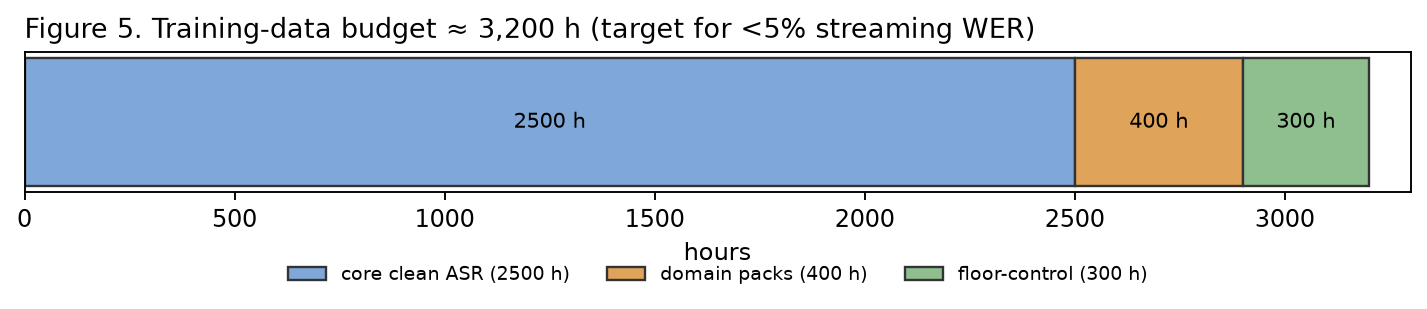
\includegraphics[width=0.9\linewidth]{figs/fig_hours.png}
\caption{Training-data budget by role.}
\label{fig:hours}
\end{figure}

\paragraph{Floor-control data generation (audio-aware).} Ordinary ASR corpora do not label
\emph{when} to fire a signal, so we synthesize that supervision. Each real clip's waveform is
\emph{read} by an energy-based VAD probe that extracts pauses, durations, leading/trailing
silence and speech rate, serialized to a compact textual ``audio card''. An LLM agent
(OpenAI-compatible endpoint; the configured model is \code{gpt-5.6-luna}) receives a batch of
$\sim$5 audio cards and produces $\sim$22 structured rows per request, grounding every row in
the given pauses. Generation runs with a concurrency of $10$ in-flight requests and a
progress bar, is resumable per batch, and every row is schema-validated (which rejects any
placement that contradicts the transcript/context --- e.g. \flag{THINK} without a preceding
\flag{EOS\_SPEECH}, or \flag{BC} before any speech) and re-rendered. The configured generation
model is \code{gpt-5.6-luna}. Figure~\ref{fig:dist} shows the enforced scenario distribution,
which is \emph{config-driven} (\code{fc.distribution}): backchannel and emotional expression
together are $\approx 26\%$ (humans backchannel often), while $\approx 45\%$ of rows still
carry \emph{no flag at all} (nothing-happens, mid-sentence pause, false-trigger, barge-in) ---
the point is to fire \emph{appropriately}, not rarely.
\begin{figure}[h]\centering
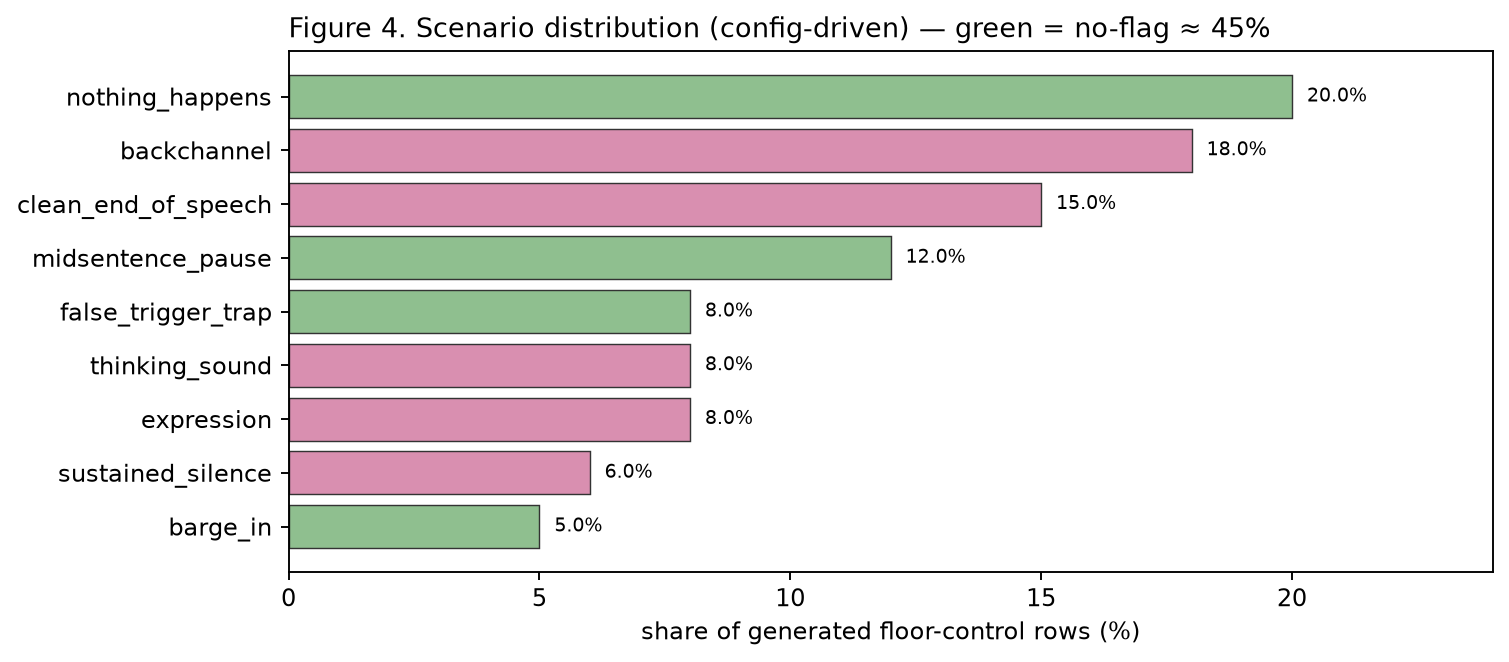
\includegraphics[width=0.86\linewidth]{figs/fig_dist.png}
\caption{Scenario distribution enforced by the generator (green = no-flag).}
\label{fig:dist}
\end{figure}

\paragraph{JSON format.} Each row is one audio-grounded example. The trainer reads
\code{audio} and \code{target\_sequence}; the rest is analysis/provenance so the data is
auditable and re-renderable. Fields: \code{id}, \code{lang}, \code{domain}, \code{scenario},
\code{audio}, \code{transcript} (plain --- the CTC target and WER reference),
\code{audio\_features} (\code{duration\_s}, \code{pauses[]}, \code{trailing\_silence\_s},
\code{speech\_fraction}, \code{mean\_energy\_db}), \code{context} (0--3 prior turns),
\code{timeline} (speech/pause segments with optional flag and surface word), and
\code{target\_sequence} (rendered, with inline flags). The renderer maps a speech segment to
its text, a \flag{BC}/\flag{THINK} pause to ``\code{<flag> surface}'', a
\flag{EOS\_SPEECH}/\flag{SILENCE} pause to ``\code{<flag>}'', and an unflagged pause to
nothing.

\paragraph{Scenario samples (generated).} Table~\ref{tab:samples} lists the nine scenarios
with the rendered target from real generated rows; note the mix of plain and emotional
backchannels and how context justifies each signal.
\begin{table}[h]\centering\small
\begin{tabular}{@{}p{3.0cm} p{4.2cm} p{6.2cm}@{}}
\toprule
Scenario & Context (prior turn) & Rendered \code{target\_sequence}\\
\midrule
nothing\_happens & --- & {\deva मुझे दवा चाहिए}\\
clean\_end\_of\_speech & {\deva Agent: आपकी क्या समस्या है?} & {\deva धन्यवाद आपका दिन शुभ हो} \flag{EOS\_SPEECH}\\
midsentence\_pause (trap) & {\deva Agent: हाँ जी बोलिए} & {\deva नमस्ते आप कैसे हैं} \ (pause, \emph{no flag})\\
backchannel & {\deva Agent: अपनी बात बताइए} & {\deva मुझे} \flag{BC} {\deva जी दवा चाहिए}\\
expression (emotional) & {\deva Agent: फिर क्या हुआ, बताइए!} & {\deva नमस्ते आप} \flag{BC} {\deva आह कैसे हैं}\\
thinking\_sound & {\deva Agent: ठीक है, बताइए} & {\deva मुझे दवा चाहिए} \flag{EOS\_SPEECH} \flag{THINK} {\deva हम्म}\\
sustained\_silence & --- & {\deva नमस्ते आप कैसे हैं} \flag{SILENCE}\\
false\_trigger\_trap & {\deva Agent: कृपया बताइए} & {\deva उम्म नमस्ते आप कैसे हैं} \ (\emph{no flag})\\
barge\_in & --- & {\deva नमस्ते आप कैसे हैं} \ (\emph{no flag})\\
\bottomrule
\end{tabular}
\caption{One generated row per scenario (Devanagari targets). Backchannel and expression
carry emotional/plain surfaces; four of nine scenarios carry no flag by design.}
\label{tab:samples}
\end{table}

\paragraph{Domain-correction record (Phase 5).} A separate record type supervises
terminology correction. Given \code{omni\_raw\_transcript} (what the acoustics literally
say), \code{context} (prior turns) and a \code{domain} tag, the target is a
\code{corrected\_transcript}, with \code{correction\_spans} listing each fix
(\code{raw}$\to$\code{fixed}, \code{reason}) and \code{chunk\_boundaries\_ms} for alignment.
The record maps cleanly onto the training row: \code{text} becomes the raw transcript (the
CTC / raw-acoustic target), \code{target\_sequence} becomes the corrected transcript (Nandi's
target), and \code{context}+\code{domain} form the decoder prefix. The split is principled:
CTC learns what the audio literally says; Nandi learns to correct it using domain and context.

\paragraph{How the agent knows the pauses (measured, not assumed).} The agent never guesses
timing. \code{fcgen.audio\_probe} reads the waveform and runs an energy-based VAD (framed RMS
in dB with a silence threshold and a minimum-pause length) to extract each internal pause's
$[\text{start},\text{end},\text{duration}]$, plus clip duration, leading/trailing silence,
speech fraction, and mean energy. These \emph{measured} values are serialized into a compact
``audio card'' that the agent must ground every row in --- it may only place flags at pause
times the audio actually contains. Solid audio evidence in, not assumptions.

\paragraph{Agent input, output, and the static/generated split (Figure~\ref{fig:agentflow}).}
The agent's input is the audio card plus the clip's \emph{real} Devanagari transcript. What is
\textbf{static} (from real data): the audio and the transcript. What is \textbf{generated} (by
the agent): the scenario, the $0$--$3$-turn context, and the flag placements with their surface
words (the timeline). The transcript is kept verbatim --- not rewritten --- which both preserves
Devanagari fidelity and saves output tokens. A merge+validate step renders the
\code{target\_sequence} (transcript with inline flags) and rejects any row that violates schema,
semantic ordering, or Devanagari purity. The collator then builds the model's \code{inputs\_embeds}
sequence and the per-chunk floor-control labels (mostly NOTHING).
\begin{figure}[h]\centering
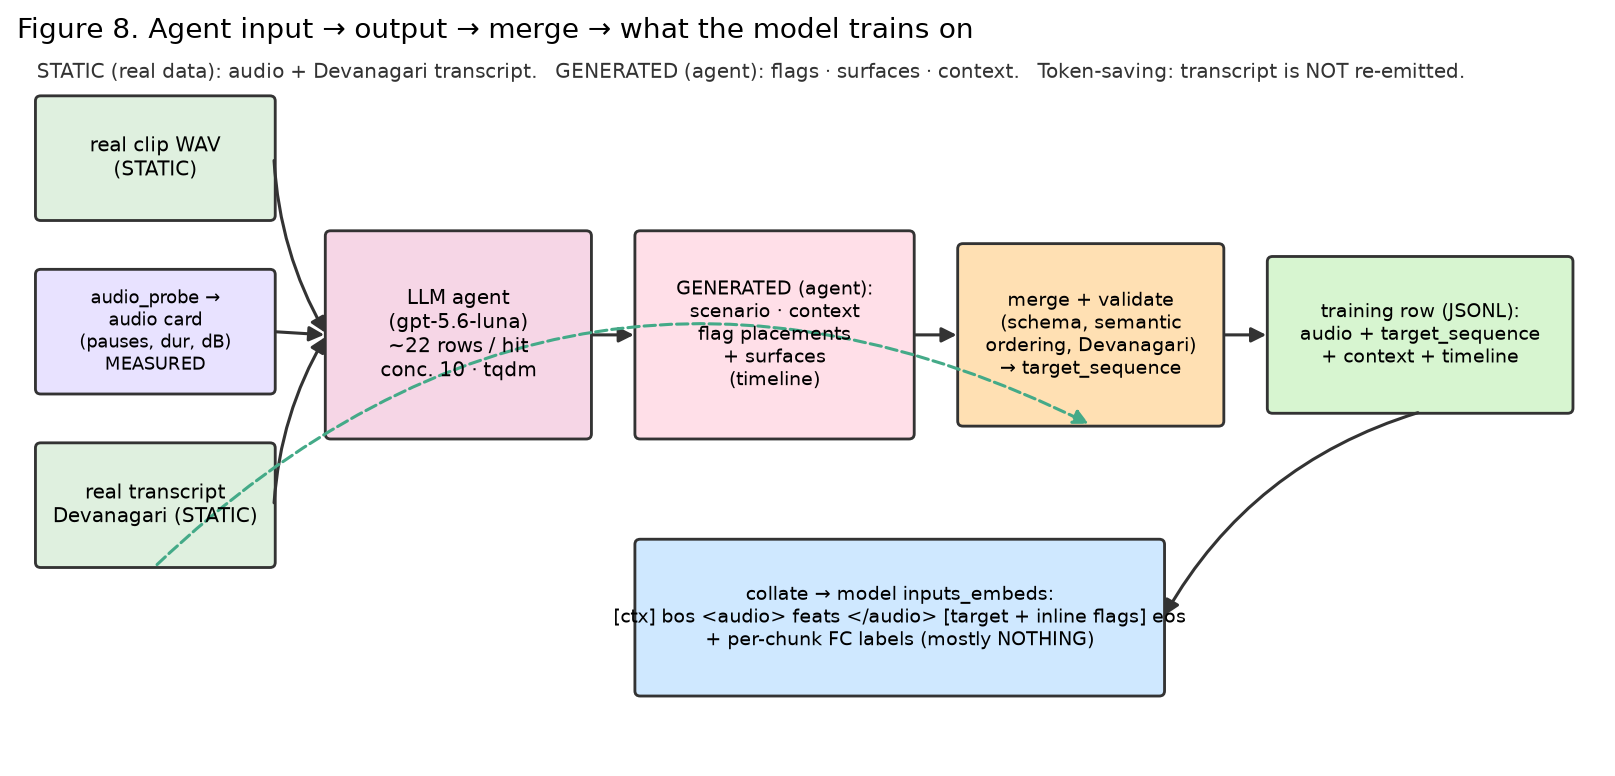
\includegraphics[width=\linewidth]{figs/fig_agentflow.png}
\caption{Agent input $\to$ generated annotations $\to$ merge/validate $\to$ training row $\to$
collated model input. Green = static (real), pink = agent-generated.}
\label{fig:agentflow}
\end{figure}

\paragraph{Token consumption (OpenAI \code{gpt-5.6-luna}).} Batching $22$ rows per call
amortizes the fixed prompt (rules + $5$ audio cards, $\approx$1.1\,k input tokens) across the
batch; with the transcript kept static, each row emits $\approx$90 output tokens (scenario,
context, timeline), so a call is $\approx$1.1\,k in $+$ $\approx$2.0\,k out. Table~\ref{tab:tok}
gives totals; keeping the transcript static saves $\approx$20--25\% of output tokens versus
re-emitting it.
\begin{table}[h]\centering\small
\begin{tabular}{@{}lrrr@{}}
\toprule
Target rows & LLM calls & input tokens & output tokens\\
\midrule
100k floor-control & $\approx$4{,}550 & $\approx$5.0\,M & $\approx$9.1\,M\\
200k floor-control & $\approx$9{,}100 & $\approx$10.0\,M & $\approx$18.2\,M\\
40k domain-correction & $\approx$6{,}700 & $\approx$4.7\,M & $\approx$4.8\,M\\
\bottomrule
\end{tabular}
\caption{Approximate OpenAI token consumption for data generation (cost $=$ tokens $\times$
per-token price). Concurrency $10$ with per-batch resume; a crash never re-spends done batches.}
\label{tab:tok}
\end{table}

\paragraph{Strict data-quality gate.} Before any training run, \code{scripts/09\_data\_quality.py}
audits a manifest and gates on hard thresholds: schema $+$ semantic-ordering validity, the
per-flag distribution and no-flag ratio, per-scenario and per-domain counts, Devanagari purity
(markup and genuine English terms stripped, then the Devanagari-letter ratio must clear $0.90$
--- this rejects romanized Hindi such as ``kaise ho''), audio existence, duration/pause sanity,
and duplicates. It exits non-zero on failure so it can block a run in CI.

\section{Streaming Input/Output Contract}
\textbf{Input:} 16\,kHz mono chunks of 320--640\,ms, plus chat context (prior turns and a
domain tag) supplied to the decoder as a \code{<hist> domain : turns </hist>} prefix.
\textbf{Output:} one record per chunk with fields \code{chunk\_id}, \code{timestamp\_ms},
\code{raw\_ctc\_transcript}, \code{corrected\_transcript}, \code{backchannel},
\code{thinking\_sound}, \code{eos\_flag}, \code{silence\_flag}. On an ordinary chunk all four
signal fields are null/false and only the transcript advances. The authoritative transcript is
\code{corrected\_transcript}, produced by \textbf{Nandi} (refreshed at end-of-turn and every
few chunks so it is stable, not flickering). \code{raw\_ctc\_transcript} is an optional,
non-authoritative low-latency draft and is \emph{off by default} --- the CTC head is used at
inference only for end-of-speech/silence timing, not to transcribe. \emph{When does a response come?} Only when the
per-chunk head's top class clearly beats NOTHING and passes the decider's threshold and
hysteresis: a backchannel mid-turn, a thinking-sound post-turn, an end-of-speech latch at
turn end, or a silence flag on a sustained gap --- otherwise the system is silent and simply
keeps transcribing.

\section{Low-Latency Design (target: end-of-turn $<100$\,ms)}\label{sec:latency}
Because the models are small ($\approx$300\,M encoder $+$ 150\,M Nandi), compute is not the
bottleneck --- on an H100 the pipeline runs many times faster than real time. The latency a
user feels after they \emph{stop speaking} has historically been dominated not by compute but
by the \emph{endpoint wait}: the silence one observes to be sure the turn is over. We remove
that wait architecturally.

\paragraph{The three levers (all in code).}
(1) \textbf{Predictive endpointing} --- the floor-control head is trained with the
\flag{EOS\_SPEECH} label \emph{shifted earlier} (\code{eos\_lead\_ms}, default $160$\,ms via
\code{events\_from\_timeline}), so it fires as the turn is \emph{finishing} rather than after a
silence timeout (\code{endpoint\_mode: predictive}). (2) \textbf{Small chunks} ---
\code{stream.chunk\_ms} $=80$ sets the reaction granularity. (3) \textbf{Zero lookahead} ---
the block-causal mask uses \code{right\_chunks: 0} (pure causal), so no future audio is
awaited; past context (\code{left\_chunks}) is free because it is already buffered.

\paragraph{Measured budget.} \code{scripts/10\_latency\_bench.py} reports per-stage p50/p95.
The end-of-turn latency is $\text{chunk\_ms} + \text{compute}$:
\begin{table}[h]\centering\small
\begin{tabular}{@{}lr@{}}
\toprule
Component & Latency\\
\midrule
Endpoint wait (predictive) & $\approx 0$ (folded into one chunk)\\
Reaction chunk (\code{chunk\_ms}) & $80$\,ms\\
Encoder on the chunk (incremental) & a few ms\\
Floor-control head (one MLP) & $<1$\,ms\\
Nandi finalize (KV-cache streaming: transcript already decoded during speech) & tens of ms\\
\midrule
\textbf{End-of-turn total} & \textbf{$\approx 80$--$120$\,ms}\\
\bottomrule
\end{tabular}
\caption{Latency budget with predictive endpointing. The reaction chunk dominates; drop
\code{chunk\_ms} to $40$ for even lower latency at some accuracy cost. Backchannels fire
\emph{during} speech at one chunk ($\approx$80\,ms).}
\end{table}

\paragraph{What it requires, and the honest tradeoff.} Two standard streaming-inference pieces
must be built (they are not in the smoke-tested code): a \emph{cache-aware incremental encoder}
(each chunk O(chunk), not O(buffer)) and \emph{KV-cache streaming decode} for Nandi (decode
tokens as audio arrives, so at end-of-turn only the tail remains). Both are well-trodden; we
have a reference (the ThinkSpark live-agent loop). The real tension is not compute but
\emph{prediction}: firing \flag{EOS\_SPEECH} within $\sim$80\,ms of the last word means
committing before a long silence confirms it, which trades a small false-cut risk for
responsiveness. We manage it with the fire threshold ($\tau_{\flag{EOS\_SPEECH}}=0.55$) and a
tiny optional lookahead; a deployment that prefers safety over speed raises the threshold or
\code{right\_chunks} to $1$. \textbf{Claim:} $\sim$80--120\,ms end-of-turn with predictive
endpointing (compute alone $<$ a few tens of ms); backchannels react within one chunk during
speech. This is at the frontier --- competitive systems sit at $200$--$500$\,ms --- so it is a
target backed by the budget above, to be confirmed on the H100 with the latency harness.

\paragraph{Does low latency hurt WER? Mostly no --- and here is exactly what does.} The
latency knobs are deliberately \emph{decoupled} from transcription accuracy:
\begin{itemize}[leftmargin=1.4em,itemsep=1pt]
\item \textbf{The $80$\,ms reaction chunk does NOT affect WER.} It only sets how often we emit
a decision. The encoder still attends over its own block (\code{chunk\_frames}$=16$, $\approx$320\,ms)
plus generous past context (\code{left\_chunks}$=4$, $\approx$1.28\,s). Those --- not the reaction
cadence --- determine transcript quality.
\item \textbf{Predictive endpointing does NOT change what is transcribed.} The encoder and
Nandi transcribe the audio regardless of when \flag{EOS\_SPEECH} fires; endpoint timing only
decides \emph{when we declare the turn over}. A premature EOS is self-healing: the
speech-resume guard (\code{StreamDecider.unlatch}) un-latches and keeps transcribing the moment
speech continues, so the tail is never dropped. The only residual risk is the downstream agent
replying a touch early --- a turn-taking nicety, not an ASR error.
\item \textbf{The one real accuracy cost is causal streaming itself} (\code{right\_chunks}$=0$,
no future context). A purely causal encoder is typically $\sim$1--3 absolute WER points worse
than the same model run offline (non-causal). Past context is free (no latency), so we use a
lot of it; if WER needs the future, \code{right\_chunks}$=1$ recovers most of the gap at the
cost of one chunk of latency --- an explicit, per-deployment dial.
\end{itemize}

\paragraph{Consolidated expectations.} Table~\ref{tab:expect} states the numbers we hold
ourselves to across the whole design (proposal targets, not results).
\begin{table}[h]\centering\small
\begin{tabular}{@{}p{5.4cm} p{3.2cm} p{4.4cm}@{}}
\toprule
Metric & Target & Notes\\
\midrule
Offline (non-causal) WER, clean test & $5$--$8\%$ & upper bound of what streaming can approach\\
\textbf{Streaming (causal) WER, clean test} & \textbf{$<5\%$ stretch, $6$--$9\%$ realistic} & the main Phase-3 gate; the honest streaming number\\
Streaming WER, real-world spontaneous & $8$--$13\%$ & $\approx$8\% would match the open SOTA (IndicConformer)\\
Streaming tax (causal vs offline) & $+1$--$3$ WER pts & shrinks with \code{right\_chunks}$=1$\\
Floor-control $F_1$ per signal & $>0.8$ & with false-fire $<2\%$ on no-flag audio\\
End-of-turn latency & $\sim$80--120\,ms & predictive endpoint; compute alone tens of ms\\
Backchannel reaction (during speech) & $\approx$1 chunk ($80$\,ms) & \\
Domain-term accuracy (Phase 5) & up, no WER regression & Nandi correction layer\\
\bottomrule
\end{tabular}
\caption{Consolidated proposal targets. Biggest lever on WER is \emph{clean data volume};
biggest risk is the Omni SSL encoder (fallback: FastConformer, Section~\ref{sec:enc}).}
\label{tab:expect}
\end{table}

\section{Key Advancements Aimed For}
\begin{enumerate}[leftmargin=1.4em,itemsep=1pt]
\item \textbf{One system, three tasks.} Transcription, live domain correction, and floor
control in a single streaming forward path, replacing a chain of separate models.
\item \textbf{Streaming-first validation.} A block-causal encoder mask from Phase 1 means the
$<5\%$ WER target is a streaming number, not an offline one that later regresses.
\item \textbf{Sub-100\,ms end-of-turn.} Predictive endpointing (Section~\ref{sec:latency})
removes the silence wait, targeting $\sim$80--120\,ms response after the user stops --- roughly
$3$--$5\times$ faster than typical $200$--$500$\,ms pipelines.
\item \textbf{Stability by construction.} A per-chunk head whose confident default is NOTHING,
trained on a large no-flag majority and guarded at inference by threshold and hysteresis, so
the agent stays quiet unless a signal is genuinely due.
\item \textbf{Audio-aware, distribution-controlled data.} An agent that reads real audio
timing and manufactures floor-control supervision with explicit traps, a config-driven
scenario mix, and semantic-validity checks; firing is further \emph{controllable at inference}
(per-signal threshold/bias/temperature) so backchannel eagerness is an operator dial.
\item \textbf{A reusable pattern.} Fusing a raw SSL encoder with a Hindi-native SLM, extending
only a handful of vocabulary tokens, scales to the remaining Indic languages and English
without redoing the expensive parts.
\end{enumerate}

\begin{thebibliography}{99}
\bibitem{omni} Meta AI. \emph{Omnilingual ASR: Open-Source Multilingual Speech Recognition for
1600+ Languages.} arXiv:2511.09690, 2025.
\bibitem{nandi} FrontiersMind. \emph{Nandi-Mini-150M} model card. Hugging Face, 2025.
\bibitem{w2v2} A. Baevski, H. Zhou, A. Mohamed, M. Auli. \emph{wav2vec 2.0: A Framework for
Self-Supervised Learning of Speech Representations.} NeurIPS 2020. arXiv:2006.11477.
\bibitem{ctc} A. Graves, S. Fern\'andez, F. Gomez, J. Schmidhuber. \emph{Connectionist Temporal
Classification.} ICML 2006.
\bibitem{hubert} W.-N. Hsu et al. \emph{HuBERT: Self-Supervised Speech Representation Learning by
Masked Prediction of Hidden Units.} IEEE/ACM TASLP, 2021. arXiv:2106.07447.
\bibitem{whisper} A. Radford et al. \emph{Robust Speech Recognition via Large-Scale Weak
Supervision (Whisper).} arXiv:2212.04356, 2022.
\bibitem{qwenaudio} Y. Chu et al. \emph{Qwen-Audio: Advancing Universal Audio Understanding.}
arXiv:2311.07919, 2023.
\bibitem{qwen2audio} Y. Chu et al. \emph{Qwen2-Audio Technical Report.} arXiv:2407.10759, 2024.
\bibitem{salmonn} C. Tang et al. \emph{SALMONN: Towards Generic Hearing Abilities for Large
Language Models.} ICLR 2024. arXiv:2310.13289.
\bibitem{vap} E. Ekstedt, G. Skantze. \emph{Voice Activity Projection: Self-Supervised Learning
of Turn-Taking Events.} Interspeech/SIGDIAL 2022.
\bibitem{indicw2v} T. Javed et al. \emph{Towards Building ASR Systems for the Next Billion Users
(IndicWav2Vec).} AAAI 2022. arXiv:2111.03945.
\bibitem{shrutilipi} K. Bhogale et al. \emph{Effectiveness of Mining Audio and Text Pairs from
Public Data (Shrutilipi).} arXiv:2208.12666, 2022.
\bibitem{lora} E. Hu et al. \emph{LoRA: Low-Rank Adaptation of Large Language Models.}
arXiv:2106.09685, 2021.
\bibitem{vaswani} A. Vaswani et al. \emph{Attention Is All You Need.} NeurIPS 2017.
\bibitem{vaani} \emph{Vaani Benchmark V1.0: An Inclusive Multimodal Benchmark Dataset for
Hindi.} arXiv:2606.21408, 2026.
\bibitem{voi} \emph{Voice of India: A Large-Scale Benchmark for Real-World Speech Recognition
in India.} arXiv:2604.19151, 2026.
\bibitem{indicconf} AI4Bharat. \emph{IndicConformer: Multilingual Conformer ASR for 22 Indian
Languages.} 2024--2026 (\code{ai4bharat/indic-conformer-600m-multilingual}).
\end{thebibliography}

\end{document}
